\section{Theorie}
\label{sec:Theorie}

\subsection{Tomographie mit $\gamma$-Strahlen}
\label{subsec:tomographie}

Die Tomographie ist ein Verfahren, welches verwendet wird, die räumliche Struktur und Zusammensetzung eines Objekts zu bestimmen, ohne dieses zu zerstören. Dabei wird das betrachtete Objekt aus verschiedenen Richtungen beispielsweise mit $\gamma$-Quanten bestrahlt, welche beim Durchdringen der Materie über Wechselwirkungen - welche in Abschnitt \ref{subsec:WW} erläutert werden - Energie an diese abgeben, sodass die Intensität abnimmt. Wird die ausgehende Intensität $I_.a$ mit der eingehenden Intensität $I_.0$ verglichen können so Querschnittsbilder verschiedener Projektionen erzeugt werden, mit Hilfe derer auf das Material des Objekts geschlossen werden kann. Da jedes Material einen bestimmten energieabhängigen Absorptionskoeffizienten $\mu$ besitzt, lässt sich $I_.a$ aus einem Objekt mit verschiedenen Materialtypen $i$ berechnen über
\begin{equation}
I_.a = I_.0\mathrm{e}^{-\sum \mu_.i d_.i}\text{,}\label{eq:Ia}
\end{equation}
beziehungsweise
\begin{equation}
\sum \mu_.i d_.i = \mathrm{ln}\left(\frac{I_.0}{I_.a}\right)\text{.}\label{eq:mu1}
\end{equation}
Dabei sind $d_.i$ die Wegstrecken die im jeweiligen Material durchquert werden müssen.
In diesem Versuch werden 3 x 3 Elementarwürfel mit $\SI{1}{\centi\meter}$-Kantenlänge in einer Ebene untersucht. Bei bekanntem $I_.0$ kann so ein Gleichungssystem zur Bestimmung der 9 Absorptionskoeffizienten aufgestellt werden:
\begin{equation*}
\mathbf{A}\vec{\mu} = \vec{I}\text{,}
\end{equation*}
wobei $\mathbf{A}$ die Designmatrix zur Beschreibung der Würfelgeometrie und der verschiedenen Projektionen, $\vec{mu}$ der 9-komponentige Vektor der Absorptionskoeffizienten und $\left(\vec{I}\right)_.i= \mathrm{ln}\left(\frac{I_.{a,i}}{I_.0}\right)$ ist.
Zur Erhöhung der Messgenauigkeit werden mehr Projektionen vermessen als Elementarwürfel vorhanden sind, um so ein überbestimmtes Gleichungssystem zu erhalten.
Eine mögliche Matrix $\mathbf{A}$ für 16 verschiedene Projektionen ist somit
\[
\mathrm{\textbf{A}} = \left(
\begin{matrix}
\sqrt{2} &  &  &  &  &  &  &  & \\
 &  & \sqrt{2} &  &  &  &  &  & \\
 &  &  &  &  &  &  &  & \sqrt{2}\\
 &  &  &  &  &  & \sqrt{2} &  &\\
1 &  &  & 1 &  &  & 1 &  &  \\
 & 1 &  &  & 1 &  &  & 1 &  \\
 &  & 1 &  &  & 1 &  &  & 1 \\
1 & 1 & 1 &  &  &  &  &  &  \\
 &  &  & 1 & 1 & 1 &  &  &  \\
 &  &  &  &  &  & 1 & 1 & 1 \\
 & \sqrt{2} &  & \sqrt{2} &  &  &  &  &  \\
 &  & \sqrt{2} &  & \sqrt{2} &  & \sqrt{2} &  &  \\
 &  &  &  &  & \sqrt{2} &  & \sqrt{2} &  \\
\sqrt{2} &  &  &  & \sqrt{2} &  &  &  & \sqrt{2} \\
 & \sqrt{2} &  &  &  & \sqrt{2} &  &  &  \\
 &  &  & \sqrt{2} &  &  &  & \sqrt{2} &  \\
\end{matrix}
\right)
\]

\begin{figure}
\centering
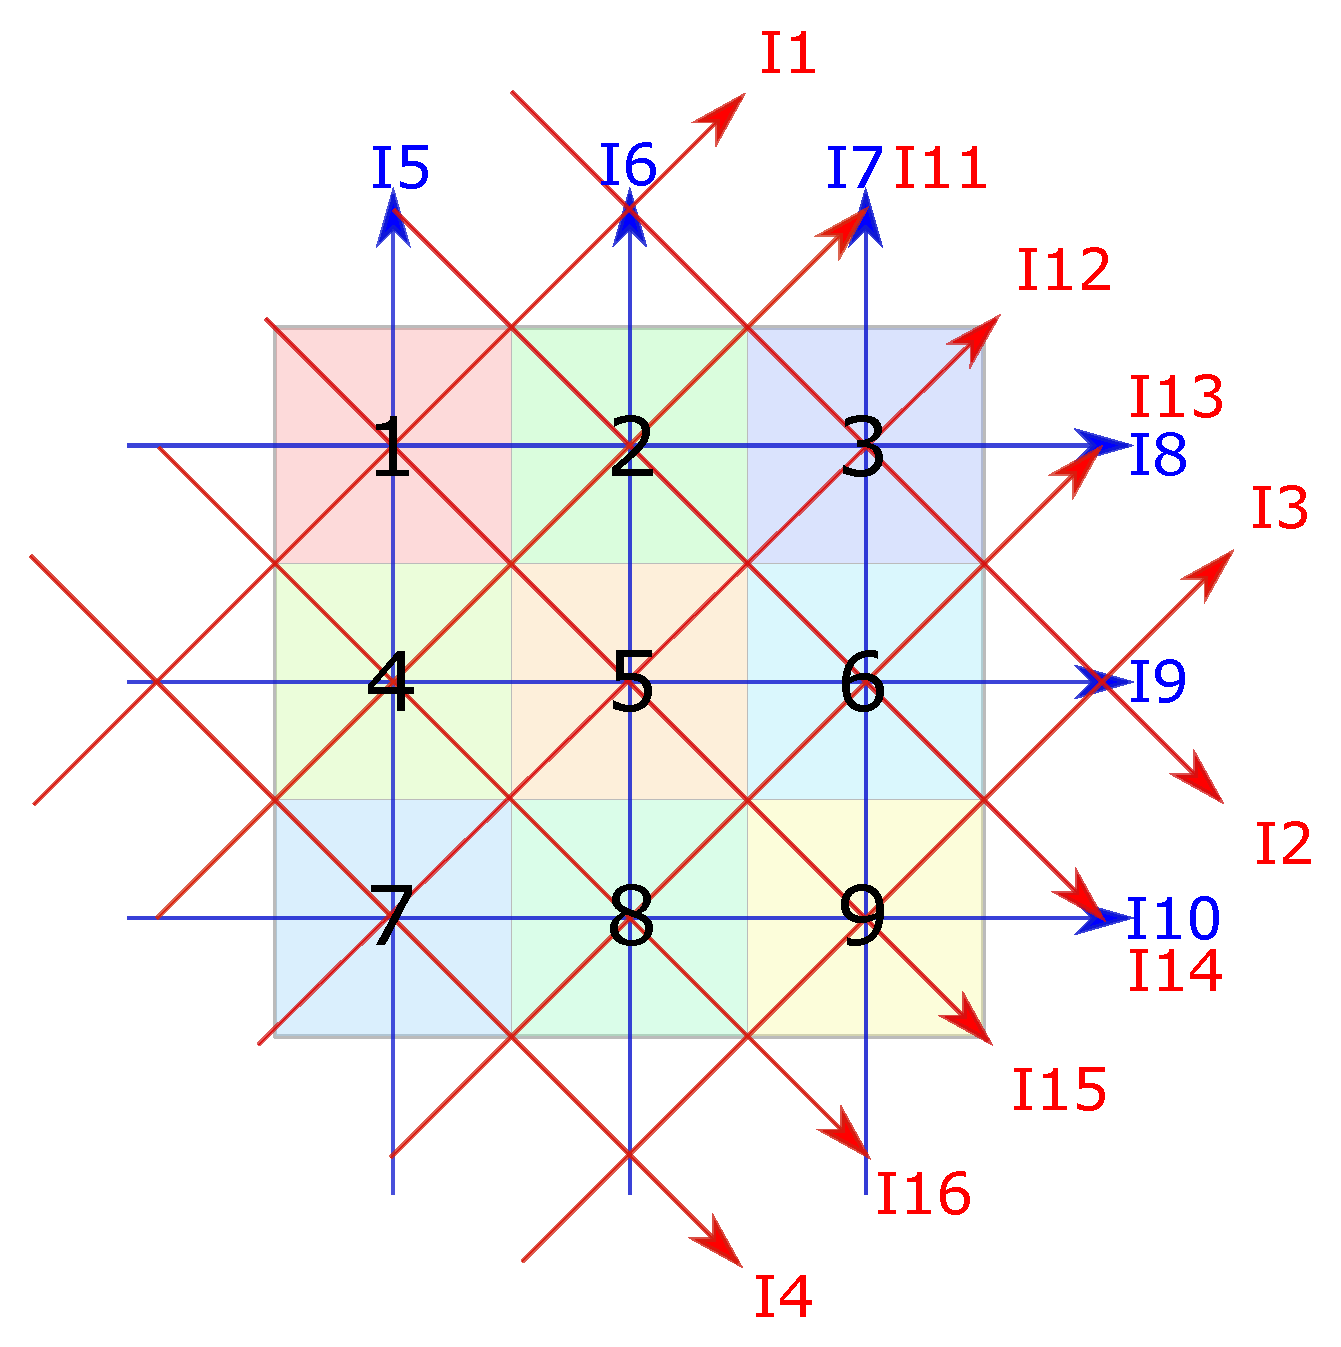
\includegraphics[keepaspectratio,width=0.6\textwidth]{content/images/Zeichnung.pdf}
\caption{Schematische Darstellung der verwendeten Projektionen.}
\label{fig:aufbau}
\end{figure}

Nach der Least-Square-Methode ergibt sich so für $\vec{\mu}$:
\begin{equation}
\vec{\mu} = (\mathbf{A}^T A)^{-1} A^T \vec{I}\label{eq:mu2}
\end{equation}

\subsection{Wechselwirkung von $\gamma$-Quanten mit Materie}
\label{subsec:WW}

Im Wesentlichen erfolgt der Energieverlust beim Durchgang von $\gamma$-Quanten durch Materie durch drei Prozesse die in verschiedenen Energiebereichen dominieren.
Eine Darstellung der Absorptionskoeffizienten der verschiedenen Prozesse in Abhängigkeit von der $\gamma$-Energie $E_.{\gamma}$, am Beispiel von Germanium sind in Abbildung \ref{fig:mus} zu sehen.

\subsubsection{Der Photoeffekt}

Für niedrige $E_.{\gamma}$ ist der äußere photoelektrische Effekt vorherrschend.
Dabei wird das eingehende $\gamma$-Quant vollständig von einem Hüllenelektron des Materials absorbiert, welches aus dem Coulomb-Potential des Kerns herausgelöst wird. Ist $E_.{\gamma}$ größer als die benötigte Austrittsarbeit $W_.A$, erhält das Elektron den Überschuss $E_.e = E_.{\gamma} - W_.A$ als kinetische Energie. Durch Stöße mit der umliegenden Materie verliert es seine Energie und kann wieder eingefangen werden, sodass die gesamte Energie im Material verbleibt.

\subsubsection{Der Compton-Effekt}

Im mittleren Energiebereich $\mathcal{O}(10 - \SI{100}{\kilo\eV})$ dominiert der Compton-Effekt, dessen Feynman-Diagramm in Abbildung \ref{fig:compton} zu sehen ist.
Dabei streut ein $\gamma$-Quant mit einem Elektron, gibt einen Teil seiner Energie ab und fliegt dann in einem Winkel $\theta$ zur Eingangsrichtung mit veränderter Frequenz weiter.
Die dabei an das Elektron abgegebene Energie berechnet sich mit der Masse des Elektrons $m_.e$ und der Lichtgeschwindigkeit $c$ über
\[
E_.e = E_.{\gamma}\left[1-\frac{1}{1+E_.{\gamma}\frac{(1-\cos(\theta)}{m_.ec^2}}\right]\text{.}
\]
Es zeigt sich das bei Vorwärtsstreuung keinerlei Energie abgegeben wird und der Übertrag im Falle von Rückwärtsstreuung maximal wird, jedoch ist selbst in diesem Fall $E_.e < E_.{\gamma}$. Es wird also nie die vollständige Energie deponiert.

\subsubsection{Die Paarerzeugung}

Im Coulombfeld eines Atomkerns oder auch eines Hüllenelektrons kann es zur Erzeugung eines Elektron-Positron-Paares kommen. Da die Energieerhaltung gilt, muss dafür $E_.{\gamma} \geq 2m_.ec^2 = \SI{1024}{\kilo\eV}$, während der Atomkern oder das Hüllenelektron als Rückstoßpartner für die Impulserhaltung benötigt werden. Da die Rückstoßenergie proportional zur inversen Masse des Teilchens ist, wird im Falle der Paarerzeugung im Elektron-Potential eine wesentlich höhere Gesamtenergie benötigt, sodass sich die Schwellenenergie für diesen Prozess auf $E_.{\gamma} \geq 4m_.ec^2$ erhöht. Das entstehende Elektron verliert seine Energie durch Stöße und kann wieder eingefangen werden, während das Positron mit einem Elektron im Material annihilieren und so zwei weitere $\gamma$-Quanten mit einer Energie von $E_.{\gamma}=\SI{512}{\kilo\eV}$ erzeugen, die entweder im Material absorbiert werden oder das Material verlassen können. 
Im Falle einer $Cs_.{55}^\text{137}$-Quelle kann dieser Prozess vernachlässigt werden, da die Energie mit $\SI{662}{\kilo\eV}$ zu gering ist.

%♥☺◙☻♦♣♠
